% FEEDBACK
%
% !TEX root = ../thesis-main.tex
%
\chapter{Feedback on lexical stress errors}
\label{chap:feedback}

%\cleanchapterquote{You can’t do better design with a computer, but you can speed up your work enormously.}{Wim Crouwel}{(Graphic designer and typographer)}

 

\begin{figure}[htb]
		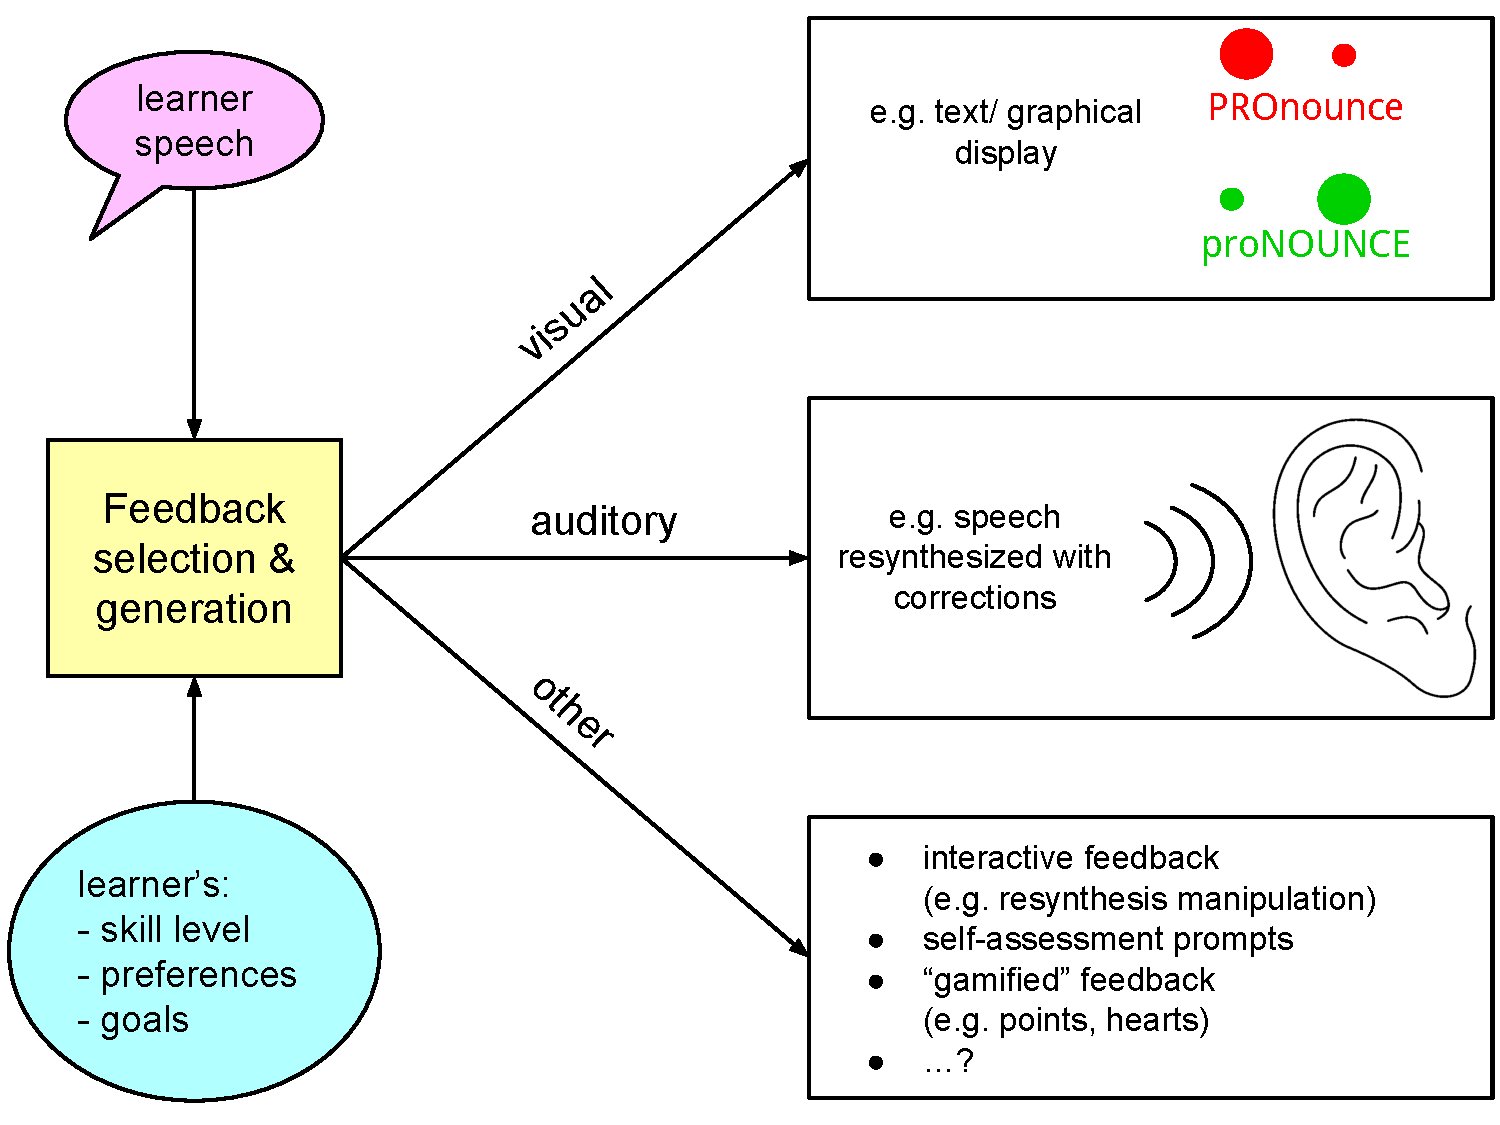
\includegraphics[width=\textwidth]{../img/feedback}
		\caption{Delivery of prosody feedback in different modalities.}
		\label{fig:feedback}
	\end{figure}

\section{Related work}

	\cite{Sitaram2011}
	\cite{Bonneau2011}
	

\section{Visual feedback}
	\subsection{Stylized text}
	\subsection{Graphical representations of prosody}
	\subsection{Visualizations of the speech signal}
	
\section{Auditory feedback}
	\subsection{Enhanced reference utterance}
	\subsection{Resynthesized learner speech}
	
\section{Alternative feedback types}
	\subsection{Metalinguistic feedback}
	\subsection{Interactive feedback}
	\subsection{Implicit feedback}

\section{Summary}